\subsection{Isoparametrische FEM}

\begin{figure}[!htbp]
\centering
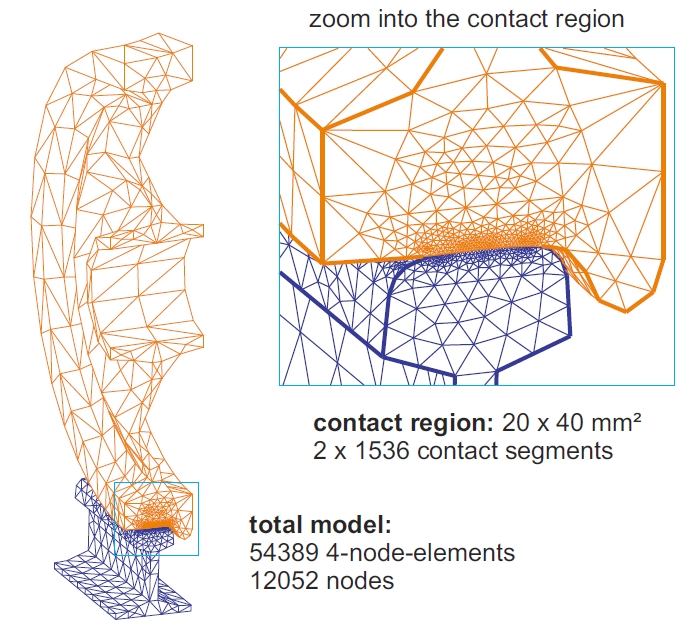
\includegraphics[width=0.75\linewidth]{files/Nackenhorst_01-22e296fb8b98cb3e9d386b83d0613561.png}
\caption[]{Geometrieapproximation am Beispiel der Diskretisierung eines Eisenbahnrades \cite{numerische_mechanik_2022}.}
\label{isogeom}
\end{figure}

Die isoparametrische Finite-Elemente-Methode ist heute der gängige Standard in FEA-Software. Erstmals erwähnt wurde die isoparametrische Finite-Elemente-Methode von I.C. Taig (britischer Luftfahrtingenieur) im Jahre 1958. Die Methode bildet die Grundlage, um komplizierte Geometrien mit gekrümmten Rändern zu modellieren. Als Beispiel sei hier die Diskretisierung in Abbildung Figure~\ref{isogeom} eines Eisenbahnrades gezeigt. In den nächsten Abschnitten werden einige Aspekte der isoparametrischen Finite-Elemente-Methode erläutert. Für einen umfassenderen Einblick sei auf die Standardwerke von \cite{zienkiewicz2005finite}, \cite{hughes2003finite} oder \cite{bathe2006finite} verwiesen.

\subsubsection{Begriffsklärung}

In der schwachen Form (\ref{weakform_03}) werden die Felder $\bm{u}_h$, $\delta\bm{u}_h$ und die Koordinaten $\bm{x}$ sowie deren räumliche Ableitungen berechnet. Das Aufstellen der Ansatzfunktionen für diese Felder ist für komplexe Geometrien nicht trivial. Daher werden die Ansatzfunktionen in einem sogenannten Elternelement definiert. Dieses wird dann auf die reale Geometrie abgebildet. Diese Abbildung wird als isoparametrische Abbildung bezeichnet. Die Abbildung wird durch die sogenannten Formfunktionen $\bm{N}$ beschrieben. Diese Formfunktionen sind in der Regel Polynome und werden in einem sogenannten Elternelement definiert. Dieses Elternelement ist ein einfaches geometrisches Objekt, wie z.B. ein Einheitsquadrat oder ein Einheitsdreieck. Die Formfunktionen sind in diesem Elternelement definiert und werden dann auf die reale Geometrie abgebildet. Dies ist in Abbildung Figure~\ref{IsoparamtericMapping} für den zweidimensionalen Fall eines Rechteckelementes dargestellt.

\begin{figure}[!htbp]
\centering
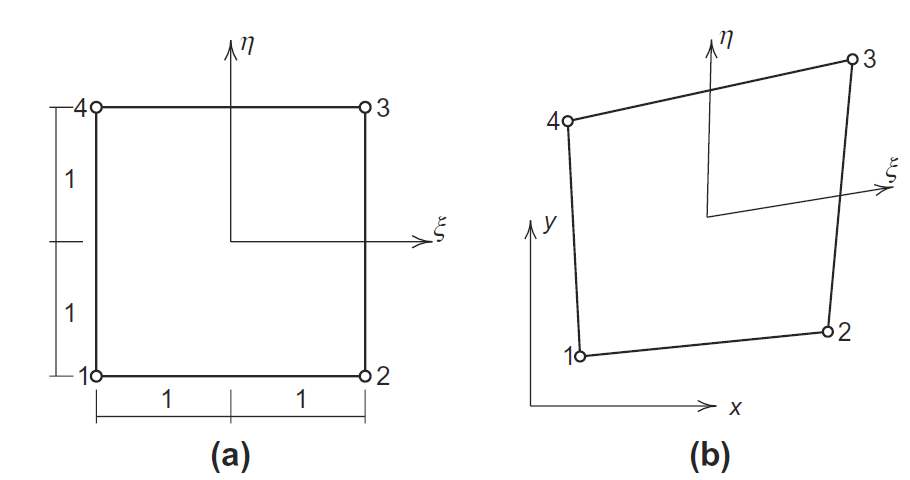
\includegraphics[width=0.75\linewidth]{files/Taylor_isoQuad-dd0d3f705ca586fcae525e52fc9aa017.png}
\caption[]{Abbildung des Elternelementes auf die reale Geometrie (\cite{zienkiewicz2005finite}).}
\label{IsoparamtericMapping}
\end{figure}

Die Abbildung des Elternelementes auf die reale Geometrie entspricht einer Koordinatentransformation. Das Elternelement wird mit den Koordinaten $\xi$, $\eta$ und $\zeta$ beschrieben, während die reale Geometrie mit den Koordinaten $x$, $y$ und $z$ beschrieben wird. Die Transformation wird durch die Abbildung $\bm{x}_h = \bm{x}_h(\xi, \eta, \zeta)$ beschrieben:

\begin{equation}
\label{geometric_mapping}
\bm{x}_h = \sum_{i=1}^{n} N_I(\bm{\xi}) \hat{\bm{x}}_I
\end{equation}

Hierbei ist $\hat{\bm{x}}_I$ der Vektor der Knotenkoordinaten und $N_I(\bm{\xi})$ die Formfunktionen des Elternelementes. Die Formfunktionen sind in der Regel Lagrange-Polynome, die die Knoten des Elternelementes interpolieren. Die Formfunktionen sind somit stückweise linear, quadratisch oder kubisch, je nach Art des Elternelementes.

Wird für die Testfunktion $\delta \bm{u}_h$ und die Verschiebung $\delta\bm{u}_h$, sowie die diskrete Darstellung der Geometrie $\bm{x}_h$ der gleiche Ansatz verwendet, so spricht man von einem isoparametrischen Element:

\begin{align}
  \delta \bm{u}_h &= \sum_{I=1}^{n} N_I(\bm{\xi}) \delta \hat{\bm{u}}_I \\
  \bm{u}_h &= \sum_{i=1}^{n} N_I(\bm{\xi}) \hat{\bm{u}}_I \\
  \bm{x}_h &= \sum_{i=1}^{n} N_I(\bm{\xi}) \hat{\bm{x}}_I
\end{align}

\begin{framed}
\textbf{Abgrenzung: weitere Parameterformulierungen}\\
Neben der isoparametrischen Formulierung gibt es auch andere Parameterformulierungen:

\begin{itemize}
\item subparametrische Formulierung: Geometrie wird mit niedrigerem Polynomgrad als die Verschiebung interpoliert
\item superparametrische Formulierung: Geometrie wird mit höherem Polynomgrad als die Verschiebung interpoliert
Beide Konzepte haben sich in der Praxis nicht durchgesetzt, wobei die superparametrische generell vermieden werden sollte (keine Konvergenz sichergestellt).
\end{itemize}
\end{framed}

\subsubsection{Berechnung der räumlichen Ableitungen}

Möchte man ein diskretisiertes Feld, z.B. $\bm{u}_h$, ableiten, so muss man über die Kettenregel die Formfunktionen ableiten:

\begin{align}
\Pd{\bm{u}_h}{\bm{x}} = \sum_{I=1}^{n} \Pd{N_I}{\bm{\xi}} \Pd{\bm{\xi}}{\bm{x}}  \hat{\bm{u}}_I \;.
\end{align}

In dieser Gleichung ist $\Pd{\bm{\xi}}{\bm{x}}$ jedoch unbekannt. Über die parametrische Darstellung der Geometrie (\ref{geometric_mapping}) kann man jedoch die Ableitung $\Pd{\bm{\xi}}{\bm{x}}$ berechnen:
\begin{align}
\bm{J} := \Pd{\bm{x}}{\bm{\xi}} & = \begin{pmatrix}
\Pd{x}{\xi} & \Pd{x}{\eta} & \Pd{x}{\zeta} \\
\Pd{y}{\xi} & \Pd{y}{\eta} & \Pd{y}{\zeta} \\
\Pd{z}{\xi} & \Pd{z}{\eta} & \Pd{z}{\zeta} 
\end{pmatrix}
=  \sum_{I=1}^{n} \Pd{N_I}{\bm{\xi}} \hat{\bm{x}}_I \\
\Rightarrow \Pd{\bm{\xi}}{\bm{x}} & = \bm{J}^{-1} \; .
\end{align}
Hier wurde die \textbf{Jacobi-Matrix} $\bm{J}$ eingeführt. Zur Berechnung der räumlichen Ableitungen der Formfunktionen werden diese einfach mit der inversen Jacobi-Matrix multipliziert:

\begin{equation}
\label{ableitungFormfunktion_03}
\Pd{N_I}{\bm{x}} = \Pd{N_I}{\bm{\xi}} \Pd{\bm{\xi}}{\bm{x}} = \Pd{N_I}{\bm{\xi}} \bm{J}^{-1} \; .
\end{equation}

\begin{framed}
\textbf{Bedeutung der Jacobi-Matrix}\\
Die Determinante der Jacobi-Matrix $\det(\bm{J})$ wird als \textbf{Jacobian} bezeichnet und stellt ein wichtiges Ma$\beta$ für die Qualität der Elementform dar. Eine Jacobi-Determinante von Null bedeutet, dass die Elementform singulär ist und die Ableitung der Formfunktionen nicht mehr eindeutig definiert ist. Es ist daher wichtig, dass die Jacobi-Determinante in dem gesamten Element positiv ist. Eine Jacobi-Determinante in der Nähe von 1 ist ideal, während Werte weit von 1 entfernt auf verzerrte Elemente hinweisen. Negative Werte der Jacobi-Determinante sind ebenfalls problematisch und sollten vermieden werden. Hier hat sich das Element selbst durchdrungen. Solche Elemente fügen dem System Energie hinzu und verfälschen die Lösung ma$\beta$geblich.
\end{framed}

\subsubsection{Anforderungen an den Finite-Elemente-Ansatz}

Um die Finite-Elemente-Methode (FEM) effektiv anzuwenden, müssen die Formfunktionen bestimmte Anforderungen erfüllen:

\textbf{Kontinuität}:

Die Formfunktionen müssen im gesamten Bereich stetig vom Grad $C^{n -1}$ sein, wobei $n$ die höchste Ableitung ist, die in der schwachen Formulierung (\ref{weakform_03}) vorkommt. Beispielsweise erfordert die Elastizitätstheorie $n=1$, was bedeutet, dass der Ansatz $C^0$-stetig sein muss. Insbesondere muss diese Stetigkeit über die Elementgrenzen hinweg gewährleistet sein. Beim Balkenelement trat die Krümmung (2. Ableitung der Durchbiegung) in der schwachen Form auf. Deshalb muss der Ansatz für das Balkenelement $C^1$-stetig sein.

\textbf{Vollständigkeit}:

Die Formfunktionen müssen die exakte Lösung approximieren können, wenn die Anzahl der Elemente gegen unendlich geht. Dies stellt sicher, dass die numerische Lösung mit zunehmender Verfeinerung des Netzes immer genauer wird.

\textbf{Eindeutigkeit}:

Die Formfunktionen müssen eindeutig sein, d.h., es darf keine lineare Abhängigkeit zwischen den Formfunktionen geben. Diese Eigenschaft ist entscheidend, um sicherzustellen, dass die Lösung der Gleichungen eindeutig bestimmt ist.

Diese Anforderungen sind essenziell, um die Genauigkeit und Zuverlässigkeit der FEM-Lösungen zu gewährleisten. Sie stellen sicher, dass die numerischen Ergebnisse physikalisch sinnvoll und mathematisch korrekt sind und dass die Methode gegen die analytische Lösung konvergiert.

Für diese drei Anforderungen existiert auch eine ingenieurmä$\beta$ige Deutung, die im Folgenden beschrieben wird.

\begin{figure}[!htbp]
\centering
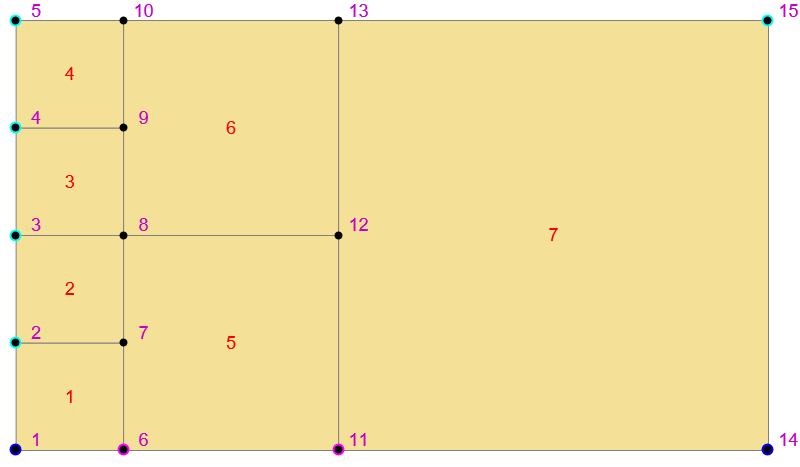
\includegraphics[width=0.75\linewidth]{files/NonConforming_Mesh_0-a479aa456cf524d92a168b6991747316.png}
\caption[]{Verletzung der Stetigkeitsanforderung in der Finite-Elemente-Methode.}
\label{Stetigkeit_01}
\end{figure}

Die Forderung der Stetigkeit über die Elementgrenzen hinweg wird über eine konforme Vernetzung sichergestellt. Ein typisches Beispiel zur Veranschaulichung dieser Anforderung ist die Elementierung mit 4-Knoten-Rechteckelementen. Betrachten wir eine eingespannte Scheibe, die einer Zugbelastung ausgesetzt ist. Um die Schnittkräfte genauer zu erfassen, wird das Netz in Richtung der Einspannung verfeinert. Dies soll die Behinderung der Querkontraktion besser erfassen. Allerdings führt diese Netzverfeinerung in einigen Fällen zu unzulässigen Klaffungen im deformierten Netz.

Die Ursache für diese unzulässigen Klaffungen liegt in der Zuordnung der Knoten zu den Elementen. In diesem Beispiel werden die Knoten 7, 9 und 12 nur zu zwei Elementen zugeordnet. Die Elementkante von Element 5, 6 und 7 wird nicht an die Deformation der genannten Knoten gekoppelt. Diese fehlerhafte Zuordnung führt dazu, dass die Schnittkräfte in der Nähe von Inkompatibilitäten nicht korrekt berechnet werden.

\begin{figure}[!htbp]
\centering
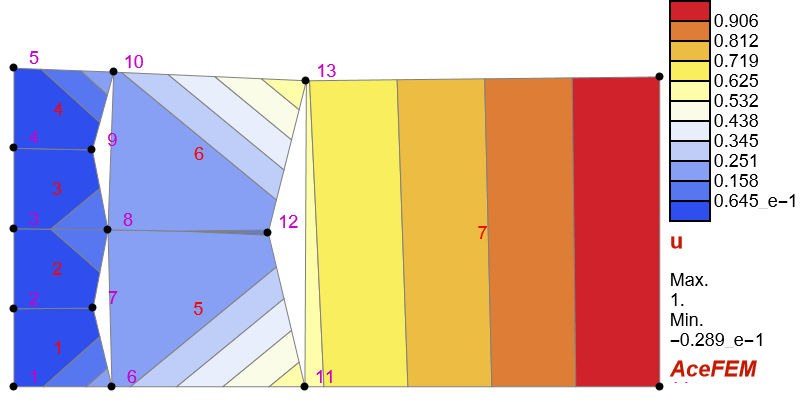
\includegraphics[width=0.75\linewidth]{files/NonConforming_Mesh_0-d55b1d7d132d2ca41b6cb0a474d78e2a.png}
\caption[]{Verschiebungsfeld bei einer nicht-konformen Netzstruktur.}
\label{Stetigkeit_02}
\end{figure}

Diese lokalen Störungen klingen jedoch mit ausreichend gro$\beta$em Abstand ab, wie es das Prinzip von St. Venant beschreibt. Dieses Prinzip besagt, dass die Auswirkungen von lokalen Unregelmä$\beta$igkeiten in der Belastung oder Geometrie mit zunehmendem Abstand von der Störungsquelle abnehmen. Daher sind die Auswirkungen der Inkompatibilitäten auf die Gesamtlösung begrenzt.

Ein weiterer Fehler, der bei der Vernetzung entstehen kann, ist die Verwendung von Elementen mit unterschiedlicher Elementordnung.

\begin{figure}[!htbp]
\centering
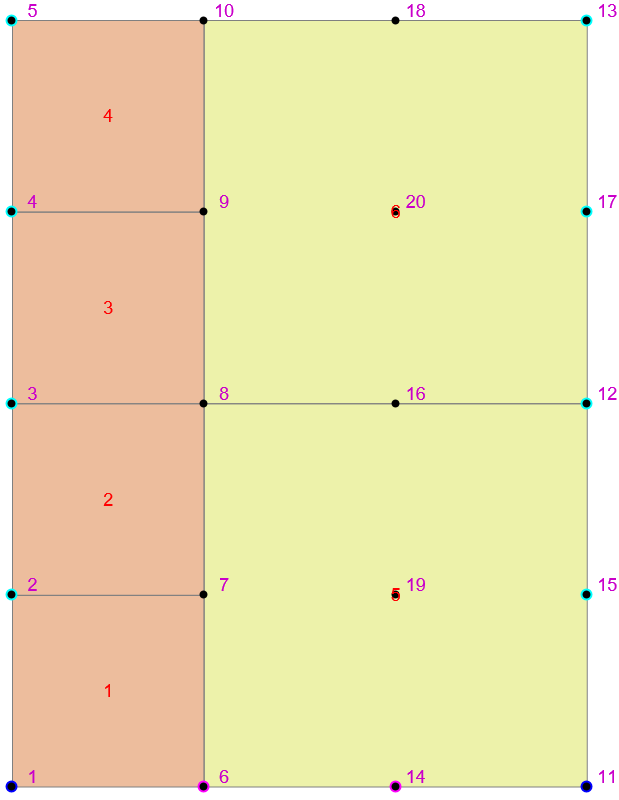
\includegraphics[width=0.5\linewidth]{files/NonConforming_Mesh_0-60bcd99bf5156e972d558f9ec97d5e1f.png}
\caption[]{Verletzung der Stetigkeitsanforderung in der Finite-Elemente-Methode durch Verwendung von Elementen mit unterschiedlicher Ordnung.}
\label{Stetigkeit_03}
\end{figure}

Auch hier ist die resultierende Verschiebung nicht korrekt. Eigentlich sollte die Verschiebung linear sein, was jedoch nicht der Fall ist.

\begin{figure}[!htbp]
\centering
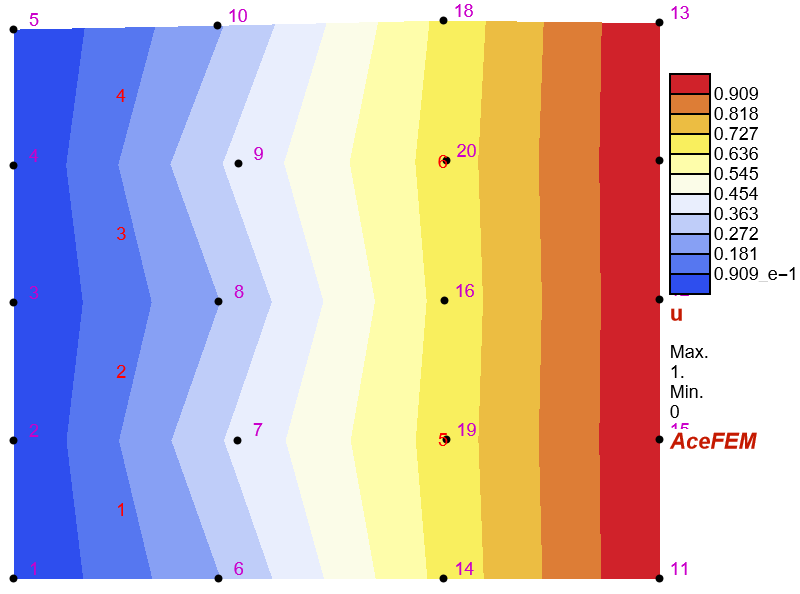
\includegraphics[width=0.75\linewidth]{files/NonConforming_Mesh_0-3212f5420fe42526cc08f008921dce3a.png}
\caption[]{Verletzung der Stetigkeitsanforderung in der Finite-Elemente-Methode durch Verwendung von Elementen mit unterschiedlicher Ordnung - Resultierendes Verschiebungsfeld.}
\label{Stetigkeit_04}
\end{figure}

Die Stetigkeitsanforderung ist von gro$\beta$er praktischer Bedeutung, da sie sicherstellt, dass die numerische Lösung physikalisch sinnvoll und mathematisch korrekt ist. Eine konforme Vernetzung, bei der die Knoten korrekt zugeordnet sind, ist entscheidend, um die Genauigkeit der FEM-Lösungen zu gewährleisten.

Um eine lokale Verfeinerung zu erzielen, kann man entweder spezielle Elemente verwenden (bei denen die entsprechenden Knoten angelegt wurden) oder man fügt eine entsprechende Zwischenschicht, wie in Abbildung Figure~\ref{Stetigkeit_05}, ein.

\begin{figure}[!htbp]
\centering
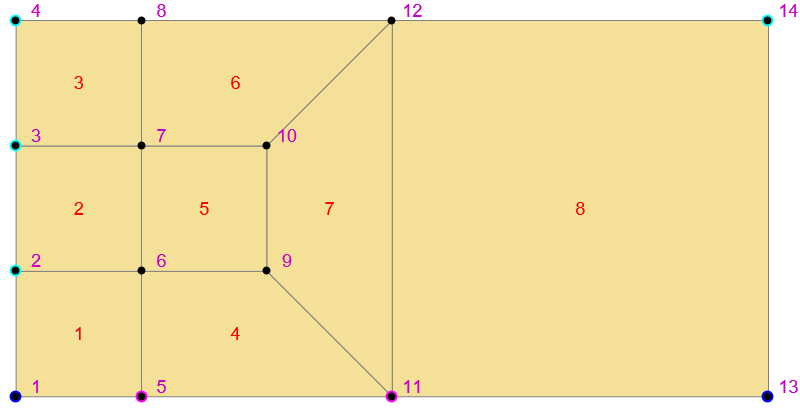
\includegraphics[width=0.75\linewidth]{files/Conforming_Mesh_01-ed2fc9715e8d4d760dd08d09cc38aea6.png}
\caption[]{Übergangselementschicht zur lokalen Verfeinerung.}
\label{Stetigkeit_05}
\end{figure}

Hierbei wird das Verschiebungsfeld durch die Zwischenschicht korrekt wiedergegeben.

\begin{figure}[!htbp]
\centering
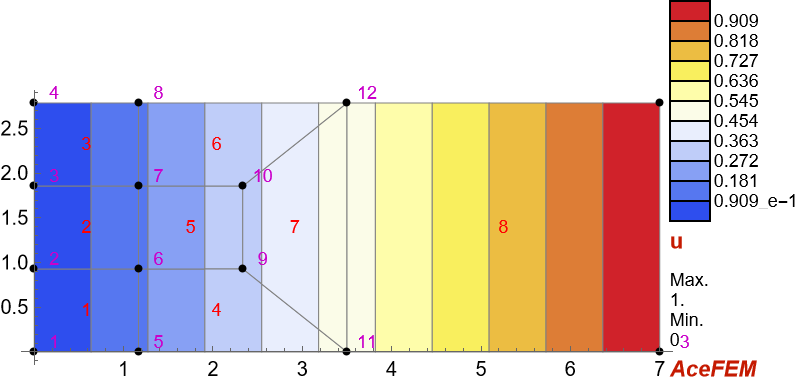
\includegraphics[width=0.75\linewidth]{files/Conforming_Mesh_02-1dadb7235cd7cceba4d6c6f0972ddf3e.png}
\caption[]{Übergangselementschicht zur lokalen Verfeinerung - Verschiebungsfeld.}
\label{Stetigkeit_06}
\end{figure}

Ein zentraler Aspekt der Vollständigkeit in der Finite-Elemente-Methode ist die Fähigkeit, Starrkörperverschiebungen darzustellen. Die Starrkörperverschiebung $\bm{u}_c = \bm{c}$ muss durch die Ansatzfunktionen $\bm{N}_I(\bm{\xi})$ exakt wiedergegeben werden können. Der mathematische Ausdruck dafür ist:
\begin{align}
\bm{u}_c & = \sum_{I=1}^{n} N_I(\bm{\xi}) \hat{\bm{u}}_I  = \sum_{I=1}^{n} N_I(\bm{\xi}) {\bm{c}} = \bm{c} \sum_{I=1}^{n} N_I(\bm{\xi}) \\
\Rightarrow \qquad 1 &= \sum_{I=1}^{n} N_I(\bm{\xi}) 
\end{align}

Diese Eigenschaft wird in der Literatur als \textbf{Partitions of Unity} bezeichnet. Die praktische Relevanz dieser Eigenschaft liegt darin, dass in Tragstrukturen die Lösung in einen Anteil der Starrkörperverschiebung und einen Anteil, der Dehnungen hervorruft, aufgeteilt werden kann. Ein Beispiel hierfür ist ein Balken: Am freien Ende ist die Verschiebung am grö$\beta$ten, der Balken jedoch erfährt hier am wenigsten Dehnung. Eine praktische Überprüfung besteht darin, dass Starrkörperverschiebungen keine Dehnungen/Spannungen hervorrufen dürfen.

Ein weiteres Beispiel zur Überprüfung der Vollständigkeit ist die Darstellbarkeit konstanter Dehnungszustände (Patch-Test). Ist ein Element in der Lage, einen konstanten Dehnungszustand darzustellen, so ist auch ein praktischer Nachweis der Konvergenz der Elementformulierung bei Verfeinerung der Vernetzung gegeben. Dies kann man sich einfach am Beispiel in Abbildung Figure~\ref{KonvergenzPatchtest} verdeutlichen. Hier werden die Schnittkräfte in einen konstanten Anteil und einen linear veränderlichen unterteilt. Mit steigender Elementanzahl wird der konstante Term der Schnittkraft dominant und ist somit der ma$\beta$gebliche Anteil für die Konvergenz.

\begin{figure}[!htbp]
\centering
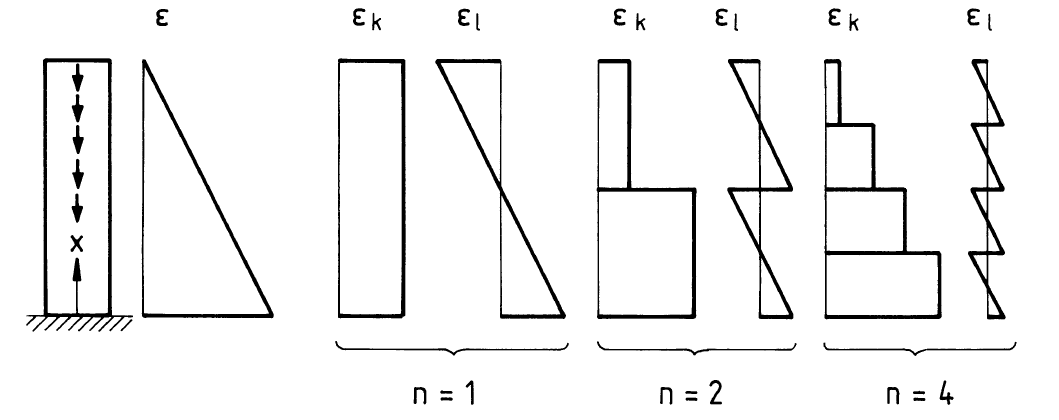
\includegraphics[width=0.75\linewidth]{files/Knothe_02-eea4e4a5abfe3ac959c4e32cca1a63d8.png}
\caption[]{Mit steigender Elementanzahl wird der konstante Term der Schnittkraft dominant (\cite{knothe1991finite}).}
\label{KonvergenzPatchtest}
\end{figure}

\begin{framed}
\textbf{Fragen zum Kapitel}\\
\textbf{Isoparametrische FEM}

\begin{itemize}
\item Welche Aussagen sind zutreffend?\begin{itemize}
\item Bei der isoparametrischen FEM wird die schwache Form auf einem uniformen Elternelement gebildet und danach auf die reale Geometrie transformiert.
\item Bei der isoparametrischen FEM werden die gleichen Ansätze bezüglich Geometrie und Verschiebung gewählt.
\item Bei der subparametrischen FEM wird die Geometrie mit einem niedrigeren Polynomgrad als die Verschiebung approximiert.
\item Nur die isoparametrische FEM ist gesichert konvergent.
\end{itemize}


\item Über welches Ma$\beta$ kann man die Qualität eines FE-Netzes quantifizieren?
\item Ist ein Element mit einer Jacobi-Determinante $\det \boldsymbol{J} < 0$ für die Berechnung zulässig?
\item Welche Anforderungen muss ein Finite-Element-Ansatz erfüllen, damit die Lösung gegen die analytische Lösung konvergiert?
\item Wie kann man die Forderung der Kontinuität des Ansatzes bei der Vernetzung verletzen?
\item Warum ist es wichtig, dass ein Finites Element Starrkörperverschiebungen korrekt darstellt?
\item Was ist ein Patch-Test? Was wird damit untersucht?
\item Was bedeutet der Begriff \textit{Partition of Unity}?
\end{itemize}
\end{framed}